\section{Experimental Method}

\subsection{Interaction Design}

\begin{figure}
\centering%
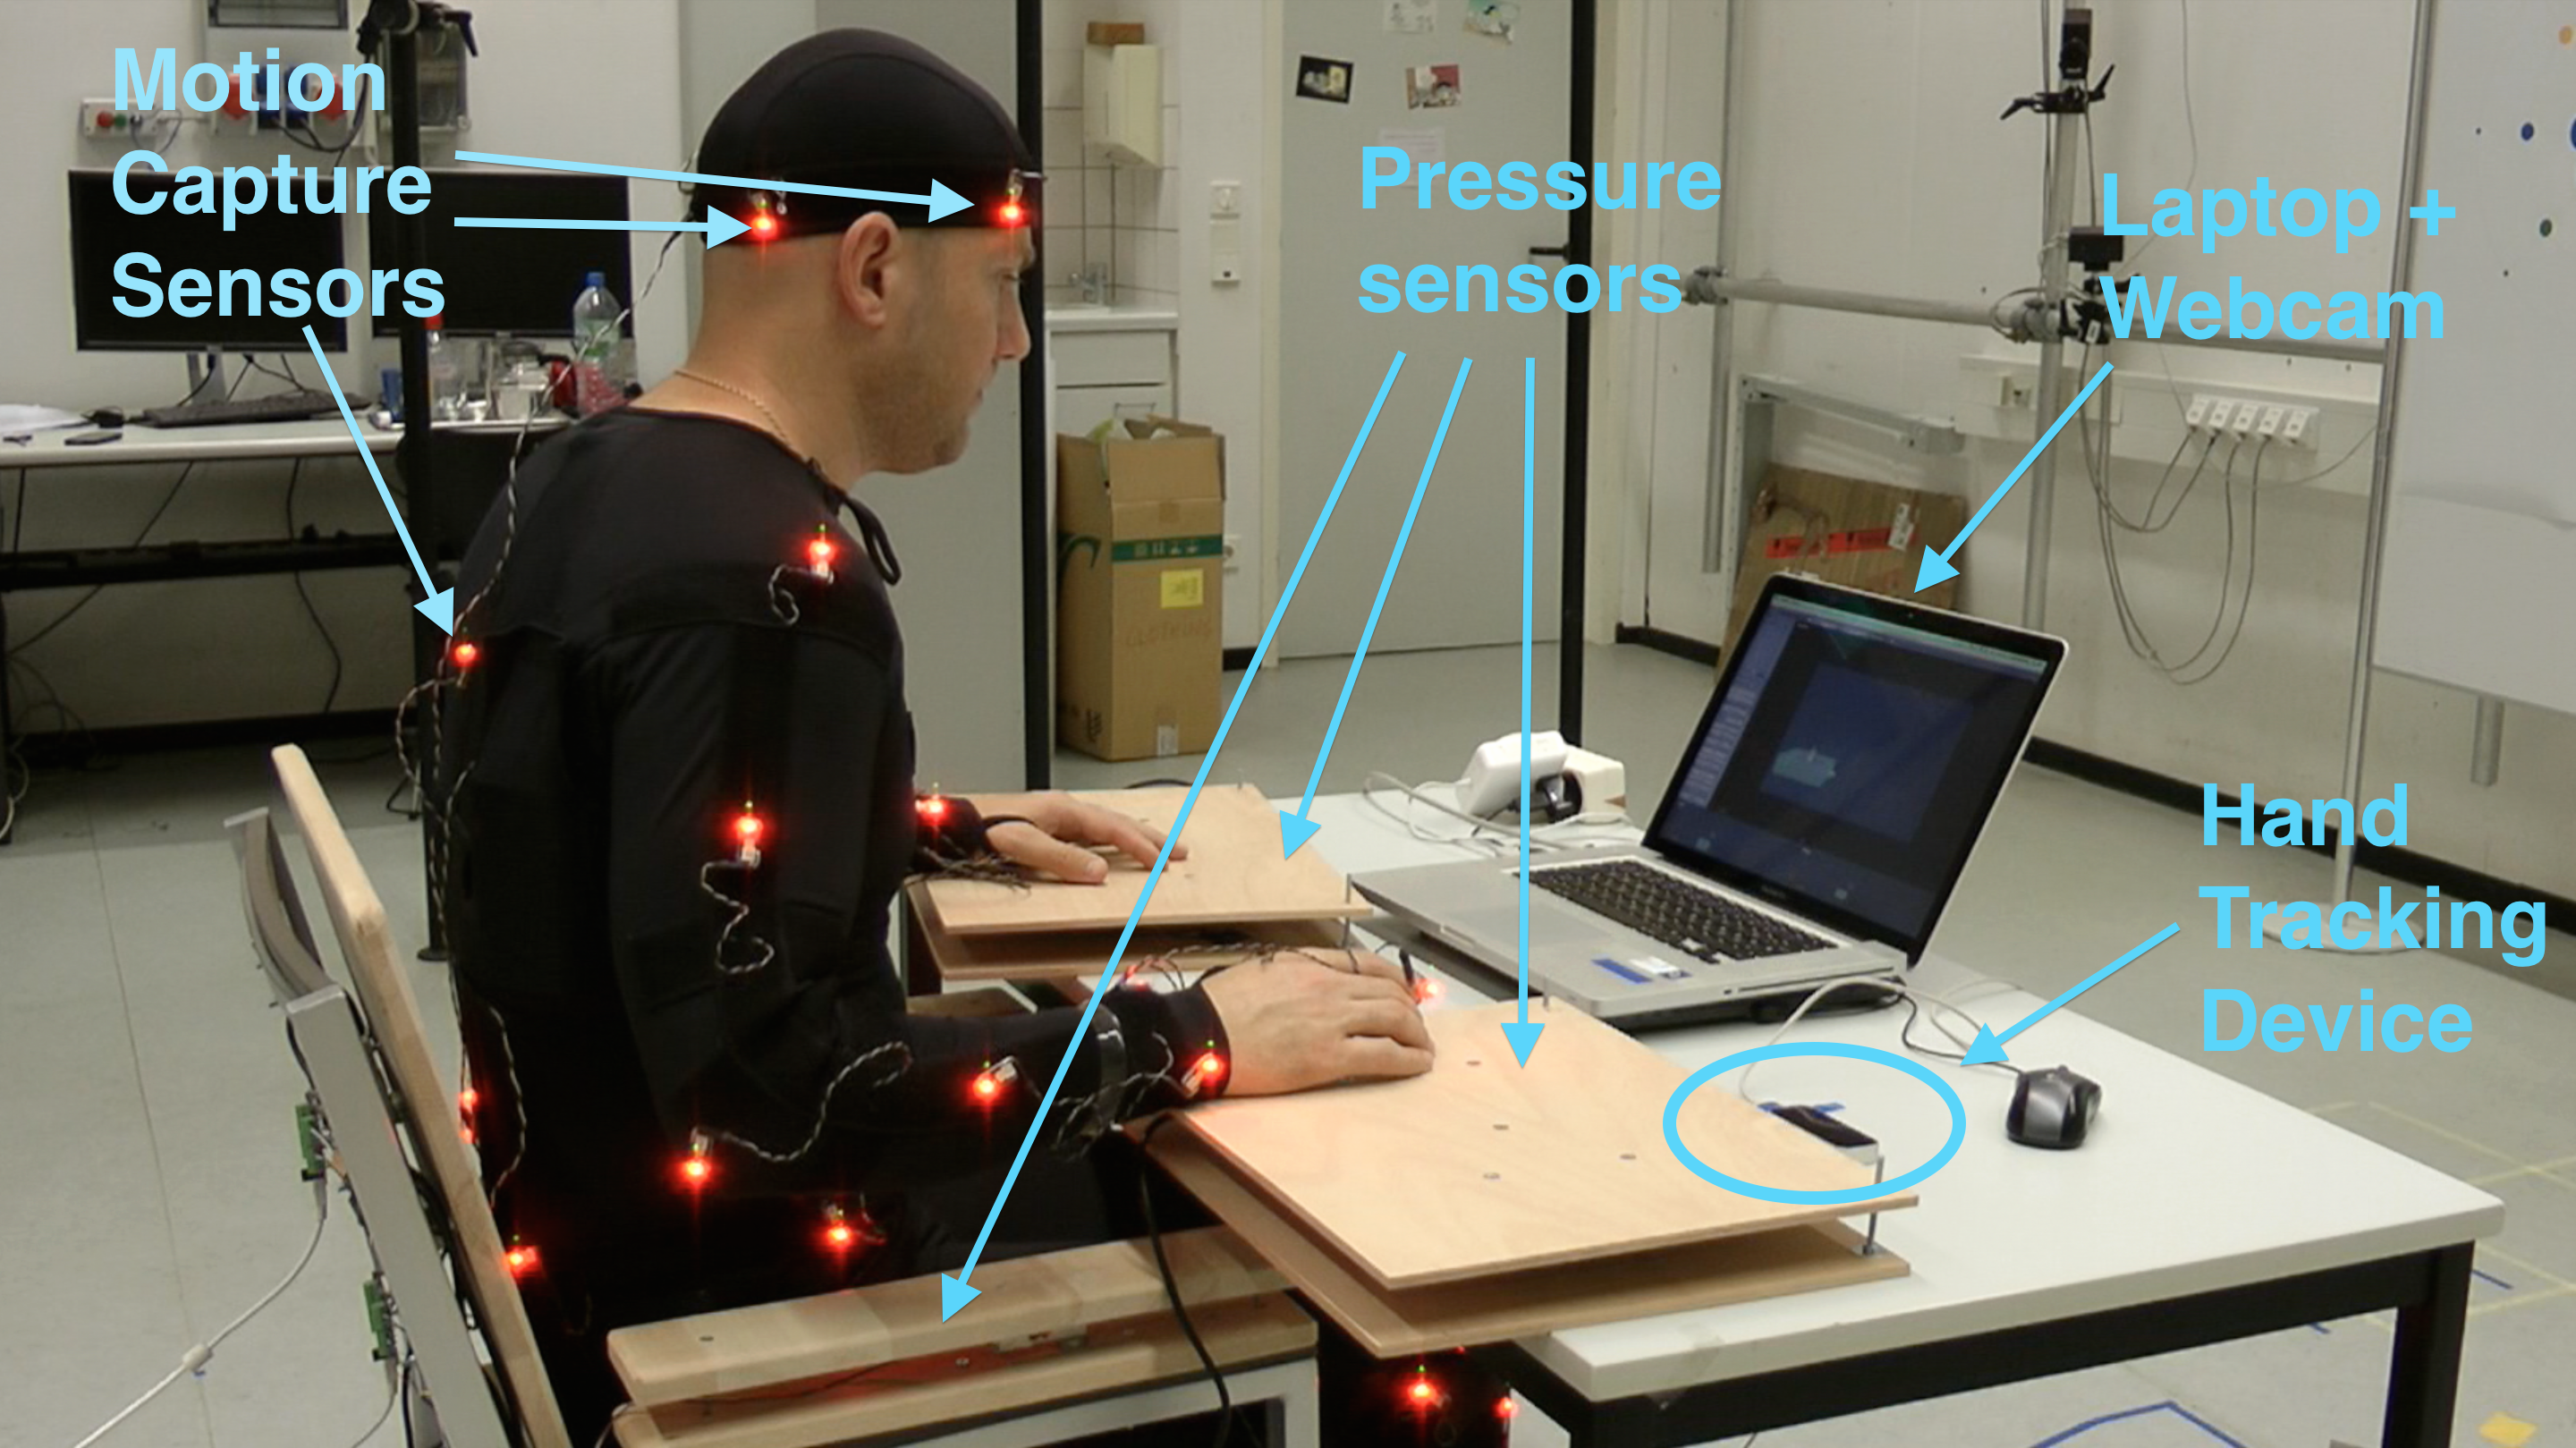
\includegraphics[width=\columnwidth]{img/user-setup}
\caption{A subject performing the docking task.}%
\label{fig:user-setup}
\end{figure}

Figure \ref{fig:user-setup} shows a picture of a user while accomplishing a \emph{docking task} \cite{zhai_quantifying_1998}, in which the subject has to use his hand to ``grab'' an object visualized in a virtual space and drop it inside a container. This task has been selected in order to lead the user to perform a set of long-lasting operations with mid-air hand movements. In the proposed setup, the subject can not accomplish the task while positioning the elbow on the surface of the desk. As in mid-air gesturing and interaction with large screens, this configuration is known to lead to muscular pain in the shoulder region (aka gorilla arm effect) \cite{hincapie-ramos_consumed_2014}.

The docking task is known to be better accomplished in presence of additional cues for the perception of depth, such as stereoscopic view \cite{boritz_study_1998}, or parallax effect \cite{Ware:1993:FTV:169059.169066}.
In order to encourage the user to involve upper body movements in the task, the movement of the head is tracked using the laptop's webcam and the inferred location of the head is used to change the viewpoint of the virtual 3D scene. The assumption is that, with parallax effect, users would have a tendency to change their stance in order to get different points of view and a better perception of depth, making the docking task easier.


\subsection{Apparatus}
The docking task has been performed on a 15 inches laptop (resolution 2880x1800, 2.4 GHz Intel Core i7, 16GB Ram).
The movement of the hand performing the docking task was tracked by a Leap Motion\footnote{\url{https://www.leapmotion.com/} -- September 25th, 2015}, whose programming interface allows for the report of pinch gestures.

The experiment was performed in a MoCap laboratory. The motions of the users were recorded at 480Hz and with 1/2mm accuracy by PhaseSpace Impulse\footnote{\url{http://www.phasespace.com/} -- September 25th, 2015} system with 12 cameras. Thirty-height active markers were distributed on the whole body of user and were attached according to anatomical landmarks to a skin-tight suit. 
External forces acting on participants body were recorded at 125 Hz with accuracy 99.8\% by a chair instrumented with 8 force sensors: 2 under the seat, 1 under backrest, 2 under armrests, 1 under footrest and 2 under movable force plates. 
The MoCap and force data were recorded by a single high-end machine (Dell Precision M4800) and synchronized with the task machine through network (\textless 1ms latency).


\subsection{Task}

\begin{figure*}%[tb]
\centering%
\includegraphics[width=\columnwidth]{img/task-performing-crop}
\includegraphics[width=\columnwidth]{img/task-accomplished-crop}
\caption{Two screenshots of the docking task as visualized on the laptop provided to the subjects. Left: the user is dragging the object inside the container. Right: the object has been correctly placed inside the container.}%
\label{fig:task-screenshots}
\end{figure*}

Figure \ref{fig:task-screenshots} shows two screenshots of the task as visualized on the screen of the laptop provided to the subject. Each trial consisted of docking a grey box inside a bigger semi-transparent red box in the virtual 3D scene (Figure \ref{fig:task-screenshots}, left).
As visual cue for the accomplishment of the task, when the grey box was correctly docked, the semi-transparent red box turned green (Figure \ref{fig:task-screenshots}, right).
In order to start the dragging procedure, the users had first to position their hand in the visibility zone of the hand-tracker and then ``pinch'' the virtual object by joining the tips of the index and the thumb. At this point, the movement of the hand in the tracking space is translated into a movement of the box in the virtual 3D scene. Users could drag the object into the container and release it by un-pinching it, i.e., separating the index and the thumb.

At the beginning of each trial, the grey object was always positioned at the center of the virtual scene, while the position of the red container was randomly selected by the system among eight fixed locations.
There was no limit to the number of times the object could be dragged and released in order to dock it correctly. It means that several drags can be performed to reach the goal.
When the trial was accomplished, the system was automatically switching to the next trial after 2 seconds.

\subsection{Experimental Design}

The docking task has been conducted on two conditions: Baseline (B) and Head Tracking (HT). In the B condition the virtual camera was fixed. In the HT condition the movement of the users' head in the real world controlled the position of the virtual camera, thus allowing for a parallax effect.
The subject had to perform as many docking operations as possible in 15+15 minutes (B + HT conditions). 
\todo[inline]{Here. We have to finally justify why we did not counterbalance. A proposal follows. Please, check-it -- FN}
The conditions have not been counterbalanced in order to present the users with a progression in the complexity of the interaction paradigm. This need emerged from the observation of the interaction of the first subjects. In the B conditions users take confidence with the gesture-based object manipulation system; in the HT condition they add the head control to the interaction.
The lack of counter-balance is a limit in the evaluation of the performances of the users in the docking task. However, since the experiment focuses on the measurement of the distribution of effort rather than of the effectiveness of the interaction method, precedence was given in effectively induce user to perform extra body movement.


The goal of the study is to measure if the stress on the shoulder reduces when the user increases the movement of the upper body.
Hence, as dependent variables we measured the quantity of movement of the head in space and a set of biomechanical indices described in detail in a later section.
\todo[inline]{or maybe now. Let's see.}
Additionally, we measured the trial completion time and the number of tasks accomplished to verify if the performance of the docking increased thanks to the parallax effect.


\subsection{Software Material}

The software driving the experiment has been programmed inside the Blender 3D authoring tool\footnote{\url{http://www.blender.org/} -- July 12th, 2016}. The task generator, the code allowing the manipulation of the 3D objects using the Leap Motion, and the logging system have been developed by the authors as Blender add-on.

In the virtual scene, the size of the box was set to 4x2x1 units, the external size of the container was set to 5,6x2,8x1,4. The location tolerance was set to 0.6 units (15\% of the longer edge) and has been imposed by the authors according to preliminary tests. At each trial, the initial position of the grey object is alway the origin of the axes, while the position of the target container is chosen randomly from 8 possible positions, given by the combination of the following translations: horizontal $\pm 6$, vertical $\pm 4$, depth $0$ or $6$.
The virtual camera is positioned at the point $0,-15.5,5.4$ and looks at the vertical axis with a rotation of 10 degrees towards the surface.

When enabled, the movement of the virtual camera is driven by the position of the face of the user. The face position is recognized through an analysis of the image captured by the webcam of the laptop. The face is recognized via a custom made application, developed in Processing\footnote{\url{https://processing.org/} -- July 12th, 2016}, which takes advantage of the OpenCV library\footnote{\url{http://opencv.org/} -- July 12th, 2016}.

% Movement proportions
%Face position is normalized
%At 60cm distance from the screen --> 20 cm on a side --> 0.5 units.
%Rotation was set to 120 degrees, it means that 0.5 on one side translates into 60 degs.
% it means that +/- 10 cm translates into +/- 30 degs rotation
%The rotation point is at 15 in front of the camera, almost around the original vertical axis.
The movement of the camera is accomplished by mapping the relative position of the face inside the webcam view to a rotation of the camera around a point in space.
After some preliminary test, the mapping was set to translate about $\pm 10cm$ of translation of the head into $\pm 30deg$ of rotation of the camera around a point set 15 units at the front (hence, close to the vertical axis).

%\todo[inline]{Actually this setup amplifies the rotation of the virtual camera with respect to a faithful simulation of the reality. It is more convenient for the user because he need less head movement to perform the same rotation, but it penalizes the experiment since it requires less motion from the user. We did not think about it in time. What to do? Skip details? - FN}

\subsection{Participants}

% code in file QuestionnaireAnalysis-RProj/analyse_profiles.R

A total of 40 subjects were recruited for the study. The data collected from the first eight subjects has been discarded because the software was still in a fine-tuning phase. Two left-handed users were discarded from the data analysis in order to focus the computation on the average stress of the muscles of the same arm. Hence, the results presented in the rest of the paper consider 30 subjects (10 Female, 20 Male), 25.53 years old on average (min=19, max=39, SD=3.91). Most of the subjects were university students in computer science.
The experiment was advertised on social networks and university mailing lists. There were no ethical issues involved in the experiment. Each participant received 10 Euros for one hour of availability, which included the time needed to wear the suit on which the markers are attached, to calibrate the motion capture, and to run the experiment.


\subsection{Procedure}

Users were sitting on a chair in front of an office desk. The chair was equipped with pressure sensors on the seat, the back, and the arm rests. Other pressure sensors were positioned on the floor, under the feet, and over the desk, under the hands. Thus we have recorded all external forces acting on a user. The laptop was positioned over the desk, in front of the user. The leap motion was positioned on the right side of the laptop in the place where typically mouse is used. However, both the laptop and the Leap were moved farther from the user, preventing the user from holding the elbow on the pressure sensor while operating mid-air gestures.
An operator assisted the users to take a comfortable position and to give instructions. Users had between two-five minutes to try the system and ask questions to the operator.
During the accomplishment of tasks, in order to avoid any disturbance, the operator was sitting about 4 meters behind the user.
